% !TeX root = ../main.tex
% Add the above to each chapter to make compiling the PDF easier in some editors.

\chapter{Implementation}\label{chapter:implementation}
In this chapter, the implementation of the system will be discussed. The system contains multiple parts working in a continuous chain. Each member of the chain is discussed individually and is displayed schematically in \autoref{fig:fullsystem}.

\begin{figure*}[htbp]
    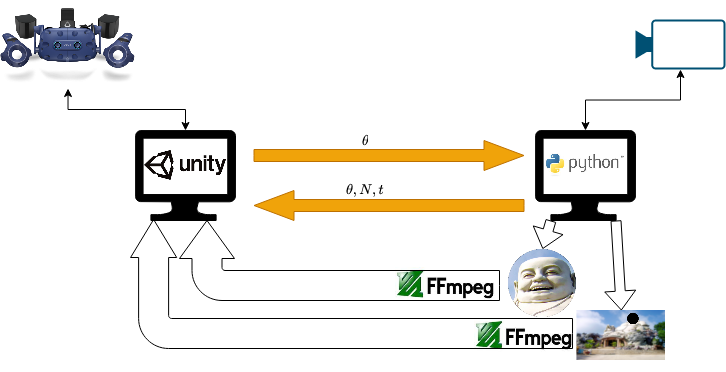
\includegraphics[width=\textwidth,height=\textheight,keepaspectratio]{logos/SystemSchematic.png}
     \caption{Schematic representation of the presented solution.}
    \label{fig:fullsystem}
\end{figure*}

\section{Foveated Streaming}\label{subsection:foveatedstreaming}
To create a foveated rendered image, locating the current gaze \(\theta\) is required. The \gls{sdk} SRanipal for the VIVE Eye Pro for Unity3D allows collecting the gaze in Unity’s update loop. The update method indicates every frame which results in a predicted \(\theta\) every 33ms when the \gls{vr} is running with 30 FPS or faster with a higher FPS. Furthermore, \(\theta\) does not correspond to the actual video coordinate system as it is guilty of the VIVEs’ system. Through RayCasting, Unity3D offers the possibility to isolate the position of a point in the view of the camera. The in-game camera calculates the hit point with a given direction, which is the current gaze. Additionally, the calculated position must be transformed to fit for the video. The predicted \(\theta\) is sent to the server through \gls{udp} as depicted \autoref{fig:fullsystem}.

 \par
In the server, a python instance runs which collects the stream of the cameras with OpenCV and crops the foveated area accordingly to the received gaze. Applying the idea of \citeauthor{Guenter2016} of streaming the images of the video as tiles instead of a complete frame, the foveated area and the peripheral area are streamed separately. FFmpeg starts with the following command and is filled with parameters explained later:
\begin{lstlisting}
    ffmpeg 
    -hwaccel cuvid 
    -y 
    -f rawvideo
    -vcodec rawvideo 
    -s  dimension 
    -pix_fmt bgr24  
    -I -
    -an 
    -vcodec hevc_nvenc 
    -maxrate speed_limit 
    -bufsize buf_size 
    -tune zerolatency 
    -pix_fmt yuv44p 
    -vsync passthrough
    -sdp_file sdp_file 
    -f rtp rtp:ip_adress:port
\end{lstlisting} 
\noindent
The command -hwaccel selects the hardware transcoder to fasten up the encoding or decoding, as it is different for each manufacturer and is in this case ‘cuvid’ to select Nvidias’ hardware transcoder . The next parameter -vcodec sets the input signal as it is unknown, because no file is given and is therefore not determined. It can be any codec like mp4, libx264 or rawvideo, meaning that it is not transcoded and is in width x height x colour-depth format. The command -s specifies the dimension of the input whereas -pix\_fmt specifies the colour format. The input given by the -I of FFmpeg is a raw image piped through the command line and thus does not exist in advance. The hyphen signals the piping. After this command, every other parameter sets the output. Since no sound exists, no sound is transmitted, which is given by -an. In addition to the specified input codec, the output codec also has to be specified. In this case, Nvidia’s Nvenc performs the H.265 encoding. Limiting the bandwidth in FFmpeg is possible with the command -maxrate. Using this command also requires using -bufsize, which controls the variability of the output bitrate. The command -tune zerolatency assures that a high encoding speed has the most importance to resume a lower quality. The YUV444p indicates the 4:4:4 chroma subsampling. The vsync parameter with the entry passthrough forces the encoder not to add interpolated images. This means that between two real frames there is no other frame added to reach a certain framerate, which is not counted correctly and therefore cannot be merged with the foveated region. The parameter -sdp\_file filename creates an sdp file stating the information about the stream and looks like the following example for an H.265 stream: 
\begin{minipage}{\linewidth}
\begin{lstlisting}
v=0
o=- 0 0 IN IP4 127.0.0.1
s=No Name
c=IN IP4 127.0.0.1
t=0 0
a=tool:libavformat 58.47.100
m=video 5004 RTP/AVP 96
b=AS:2000
a=rtpmap:96 H265/90000
\end{lstlisting}
\end{minipage}
Moreover, stated in the parameter list is the real-time transport protocol (RTP), which is a package-based protocol and is responsible for the continuous transmission of the data. The Internet Society defined it as RFC 3550 \parencite{Schulzrinne2003}. Using this protocol requires stating the sdp file as the input, specifieng the stream details.

\par
Since the predicted gaze is not 100 \% accurate, it slightly flickers even when the eye is not moving and there is a delay of the visible image, the selected foveated area is more significant than the mentioned 5$^\circ$ of the human’s view. Having an \(r = 128\) pixels resulting in a 256x256 image size worked well during the development. These images are streamed in full resolution with the highest possible quality as this is visible for the user. Oppositely, the peripheral area is compromised as much as possible without losing too many details to save bandwidth and to save computation time, as smaller images are easier to encode than larger ones. Therefore, the size of the background is reduced, resulting in a 512x256 image. This size is not precisely \(\frac{1}{4}\) of a 1920x1080 = Full HD image, and for the \gls{sr}, because the image should be dividable by 128. The resulting upscaled image is therefore 2048x1024 being in a 1:2 ratio instead of a 16:9 ratio. The reason this is necessary is explained in \autoref{subsection:superresolution}. An example of the possible result is presented in \autoref{fig:examplestream}. With the generated frame number, it is possible to connect the \(\theta\) coordinates to the frame, which becomes essential for merging both images. This step is necessary, because FFmpeg or VLC do not synchronise the frame count on the server and client side, as each side counts their frames from the beginning individually. Moreover, the coordinates cannot be parsed directly into the frame as the encoding process changes these values. The server sends the frame number, the coordinates and a timestamp as a package back to the client. This happens in parallel to the streams, as stated in \autoref{fig:fullsystem}.

\begin{figure}[htbp]%
    \centering
    \subfloat[\centering Foveated Image]{{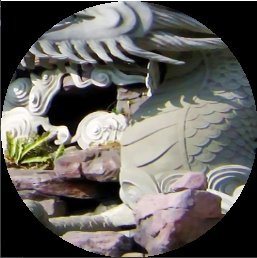
\includegraphics[width=2.56cm,keepaspectratio]{logos/FR.png}}}%
    \qquad
    \subfloat[\centering Peripheral Image]{{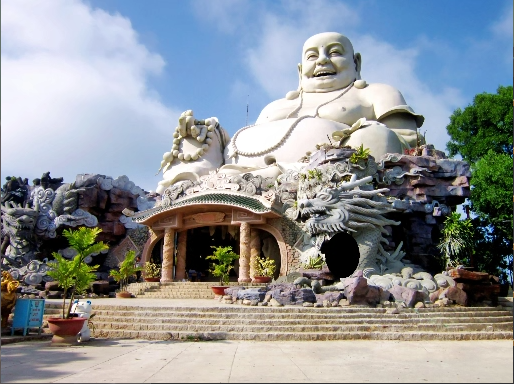
\includegraphics[width=5.12cm,keepaspectratio]{logos/peripheral.png} }}%
    \caption{Examples of the streamed images. The image is taken from the DIVK dataset \parencite{Agustsson2017}.}%
    \label{fig:examplestream}%
\end{figure}

\par
The server also tests the connection to the client to determine the available bandwidth \(\kappa\) at the beginning. This is possible since the iPerf3 is broadly available for different programming languages. This tool actively measures the maximum available bandwidth of networks. The measured bandwidth is divided by two and is the maximum available bandwidth for both the foveated and peripheral streams. The limit is inserted to the -maxrate parameter and in this scenario, the bufsize it set equal to the available bandwidth. 
\begin{center}
-maxrate \(\frac{\kappa}{2}\) -bufsize \(\frac{\kappa}{2}\)
\end{center}
\par
Back at the client-side, FFmpeg ist started with the command:
\begin{lstlisting}
    ffmpeg 
    -protocol_whitelist udp, rtp, file, pipe, crypto, data
    -hwaccel_output_format cuda 
    -probesize 32
    -analyzeduration 0
    -fflags nobuffer    
    -flags low_delay  
    -i sdp_file
    -vcodec rawvideo
    -pix_fmt bgr24
    -f image2pipe -
\end{lstlisting}
\noindent
The parameter -protocol\_whitelist is necessary for FFmpeg to use the stated protocols. The client incurs the hardware support parameter from the server as well as the flags for the low latency priority by signalling to avoid buffering and preferring a higher decoding speed. The probesize and analyzeduration parameters set the size and the duration of data which is analysed to obtain information from the stream. As this process adds some latency, it is reduced to the lowest possible value. The given sdp-file as input is generated by the server and is provided by using a weblink or by copying the file. The output of the decoding is images in the BGR colour scheme piped through the command line.
\par
The client receives both streams as well as the data package. The package contains the frame-number, the corresponding gaze coordinates and a timestamp. As the streams and data packages are not received simultaneously, synchronising the frame-number between the client and the server is required. To obtain the current number, the FPS from FFmpeg is collected, which indicates how long the decoding needs for a frame. With the received timestamp, the network delay \(\tau\) is calculated, resulting in the following formula:
\[\lambda = CurrentFrame - Offset = CurrentFrame - \frac{\tau}{\frac{1000ms}{FPS}} \]
\par
The algorithm stores the calculated frame number until FFmpeg decodes the corresponding frame. At this time, the peripheral area is resized to its original size, which is performed classically with a bicubic interpolation or \gls{sr}, and it is compared by quality and latency. Afterwards, OpenCV merges the foveated and the peripheral region at the corresponding coordinates. As the calculation is multithreaded, the merged images may appear in the wrong order, but as the processing takes more or less equally, it rarely happened during the development. That late processed images were shown to the user was prevented by checking the frame number. 

\begin{figure*}[htbp]
    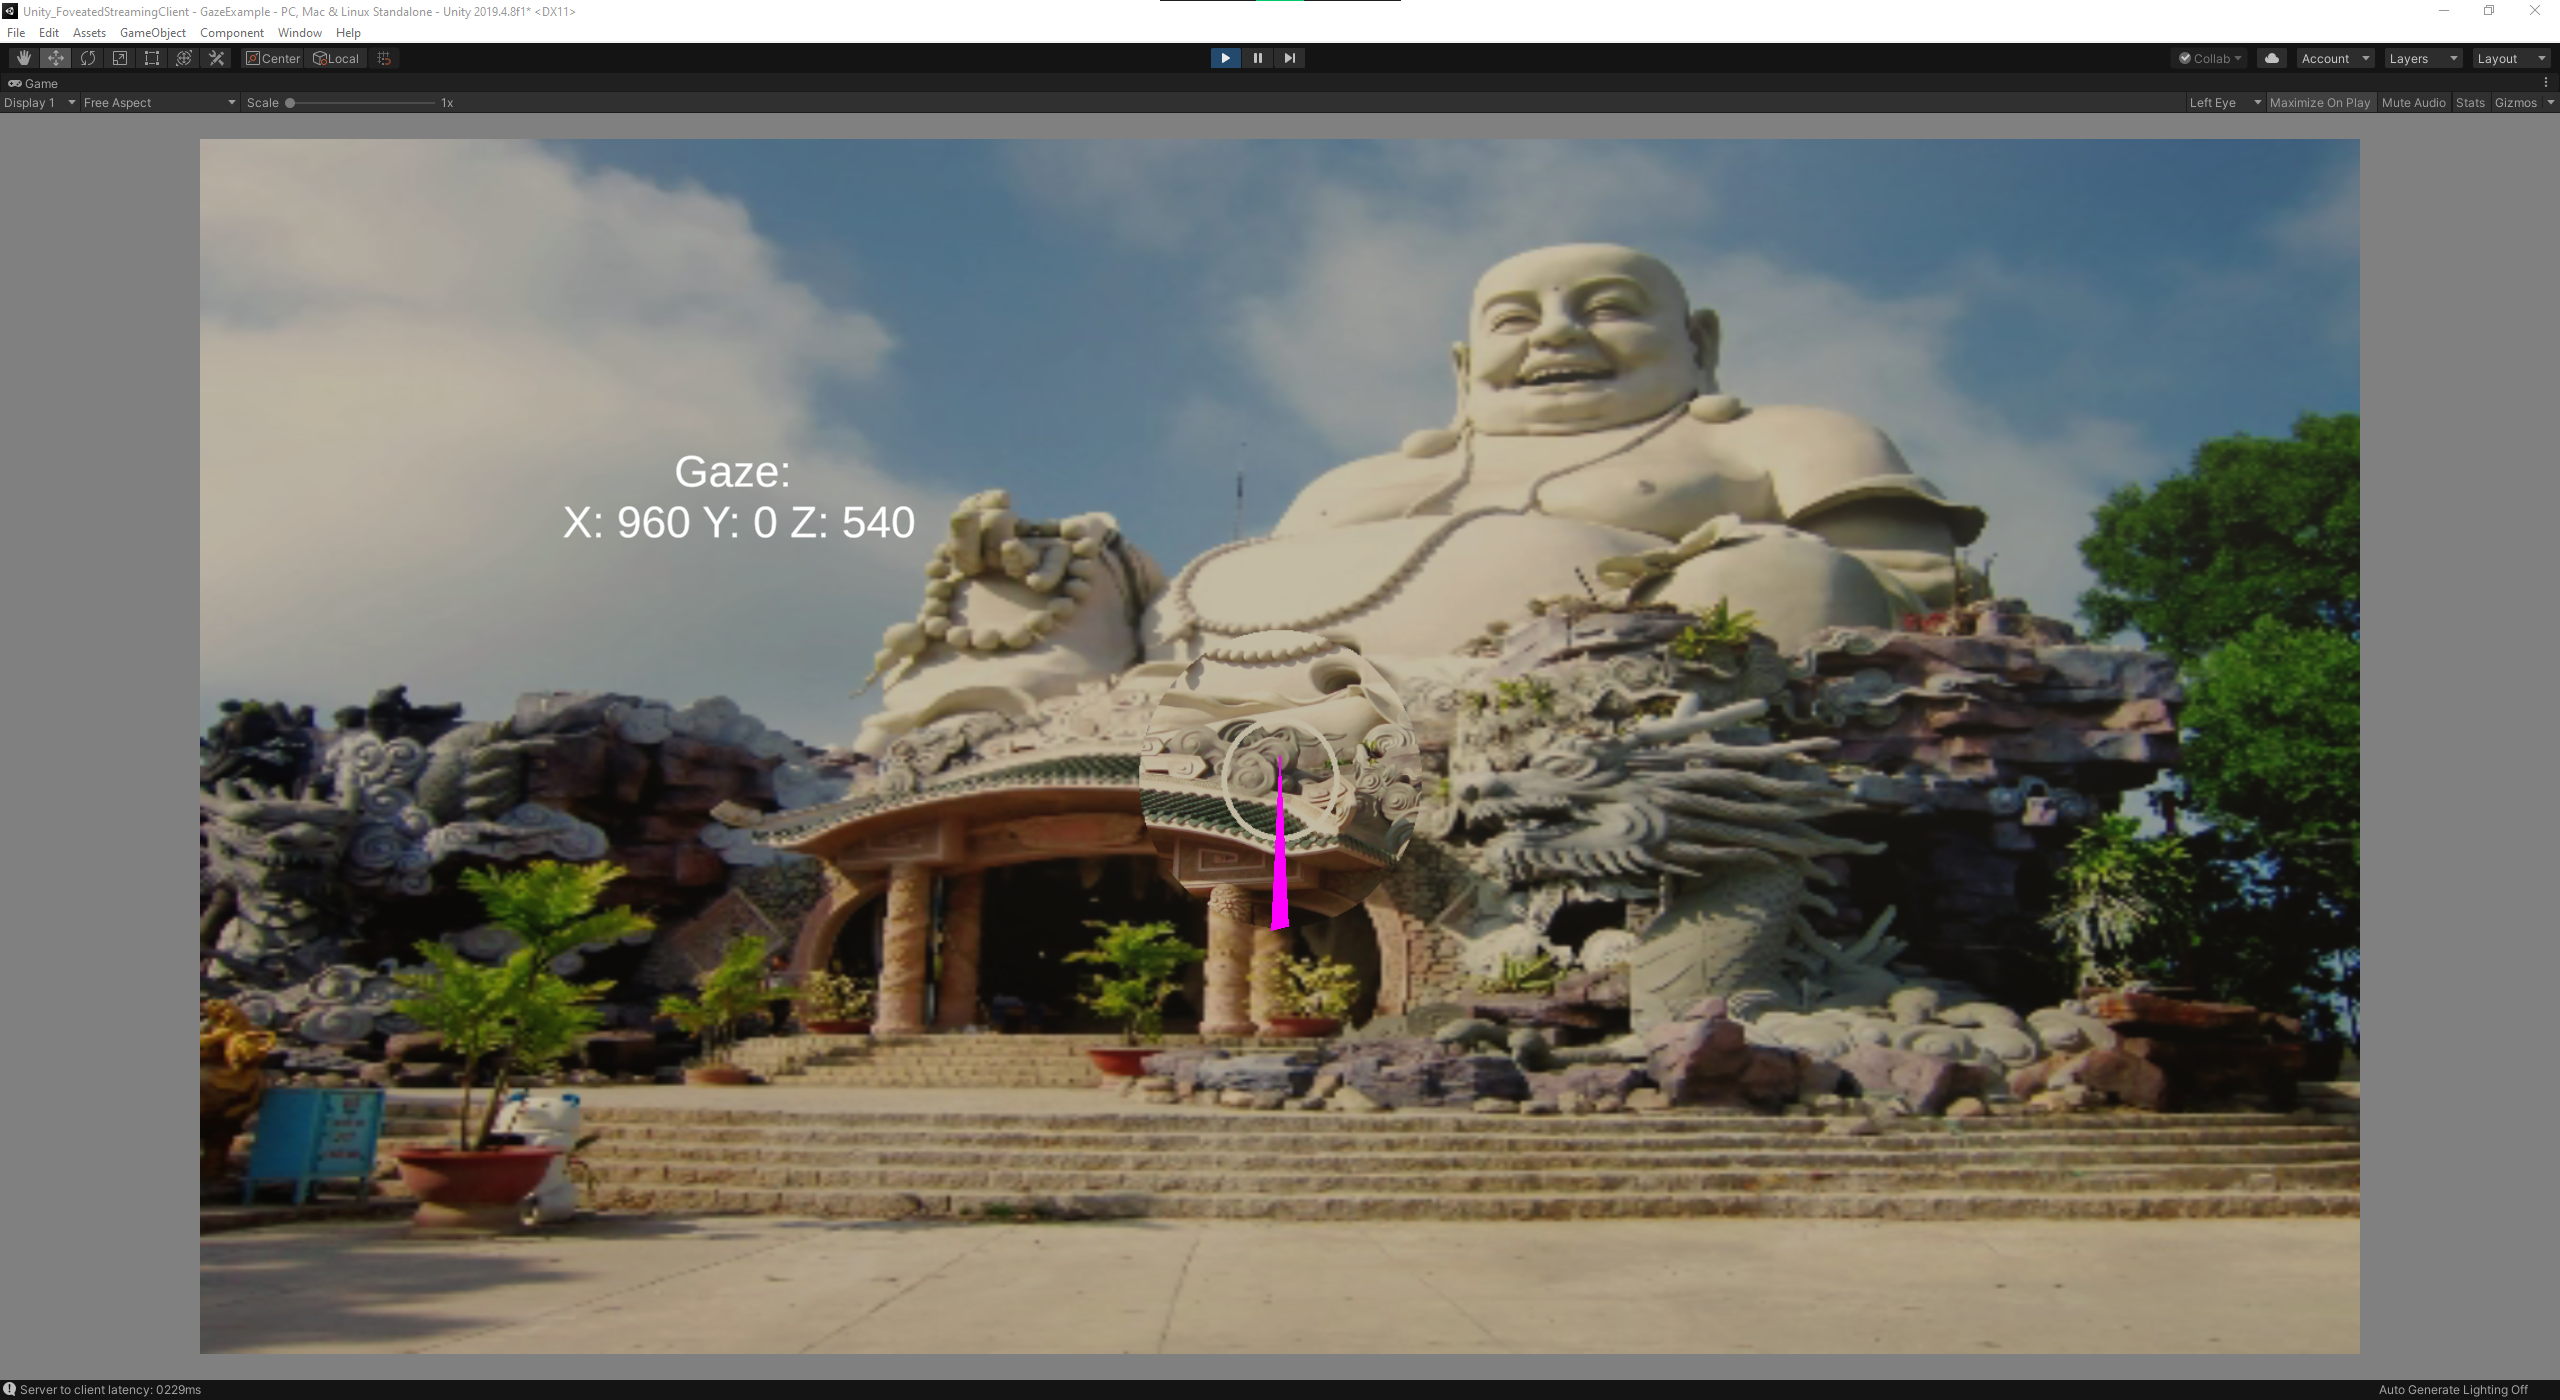
\includegraphics[width=\textwidth,height=\textheight,keepaspectratio]{logos/unity3d.png}
     \caption{Example view of a received image in 3D. The pink arrow displays the current gaze, whereas the white circle indicates the received gaze. The image is from the DIVK dataset \parencite{Agustsson2017}}
    \label{fig:unity3dgameview}
\end{figure*}

\section{Visualization}\label{subsection:visualization}
Unity3D displays the foveated rendered image on a plane in the 3D view. The result is visible in \autoref{fig:unity3dgameview}. Unity3D requires using a 3D object as a video screen, as the Raycast does not hit pure UI elements which would result in not having the correct coordinates. Additionally, the image is stretched as the image is mapped from a 3D game view to a 2D image.

\section{Superresolution}\label{subsection:superresolution}
To increase the size of an image, the missing pixels in between have to be calculated. Image libraries estimate these unknown pixels with different interpolation techniques such as the bicubic method, which uses 4x4 pixel squares to determine a new pixel by identifying the coefficients of the pixels in the square. This method is a considerable operation, and the nearest neighbour interpolation takes the average of the neighbours and is consequently faster. These methods work for each image individually, leading to recalculate the same pixels again and again when the image looks similar, as the algorithm has no memory about the preceding images. The example in \autoref{fig:comparison} shows that the bicubic interpolation has smoother edges than the liner one, but it is much weaker in terms of quality than the original high-resolution image. Another possibility is to use \gls{ml}-based \gls{sr}. \glsfirst{ml} has the advantage to learn the statistics of thousands of images. In this scenario, the focus is primarily on time rather than on quality, as the peripheral area is not in the user’s gaze and, therefore, is seen more schematically. Alternatively, when the available bandwidth is low, the pixelated image becomes visible for the user and should be avoided. Thus, the goal is to keep a minimum level of quality balanced with the latency. Facebook created with DeepFovea, which is a \gls{gan} capable of performing the \gls{sr} with four Nvidia Tesla V100 in under 10ms \parencite{Kaplanyan2019}. Additionally, it took less than 1ms to calculate a sparsified matrix of the current game view. However, this amount of graphic cards were not available. Moreover, calculating the 5D matrix as described in FaceBooks’ paper, is not usable as the image is streamed and decoded in the BGR colour scheme, which has only three dimensions. In contrast, the \gls{srgan} is capable of performing \gls{sr} with a good result but is slower as many more layers are used. Therefore, a mix of both of them is the right approach.


\begin{figure*}[htbp]
    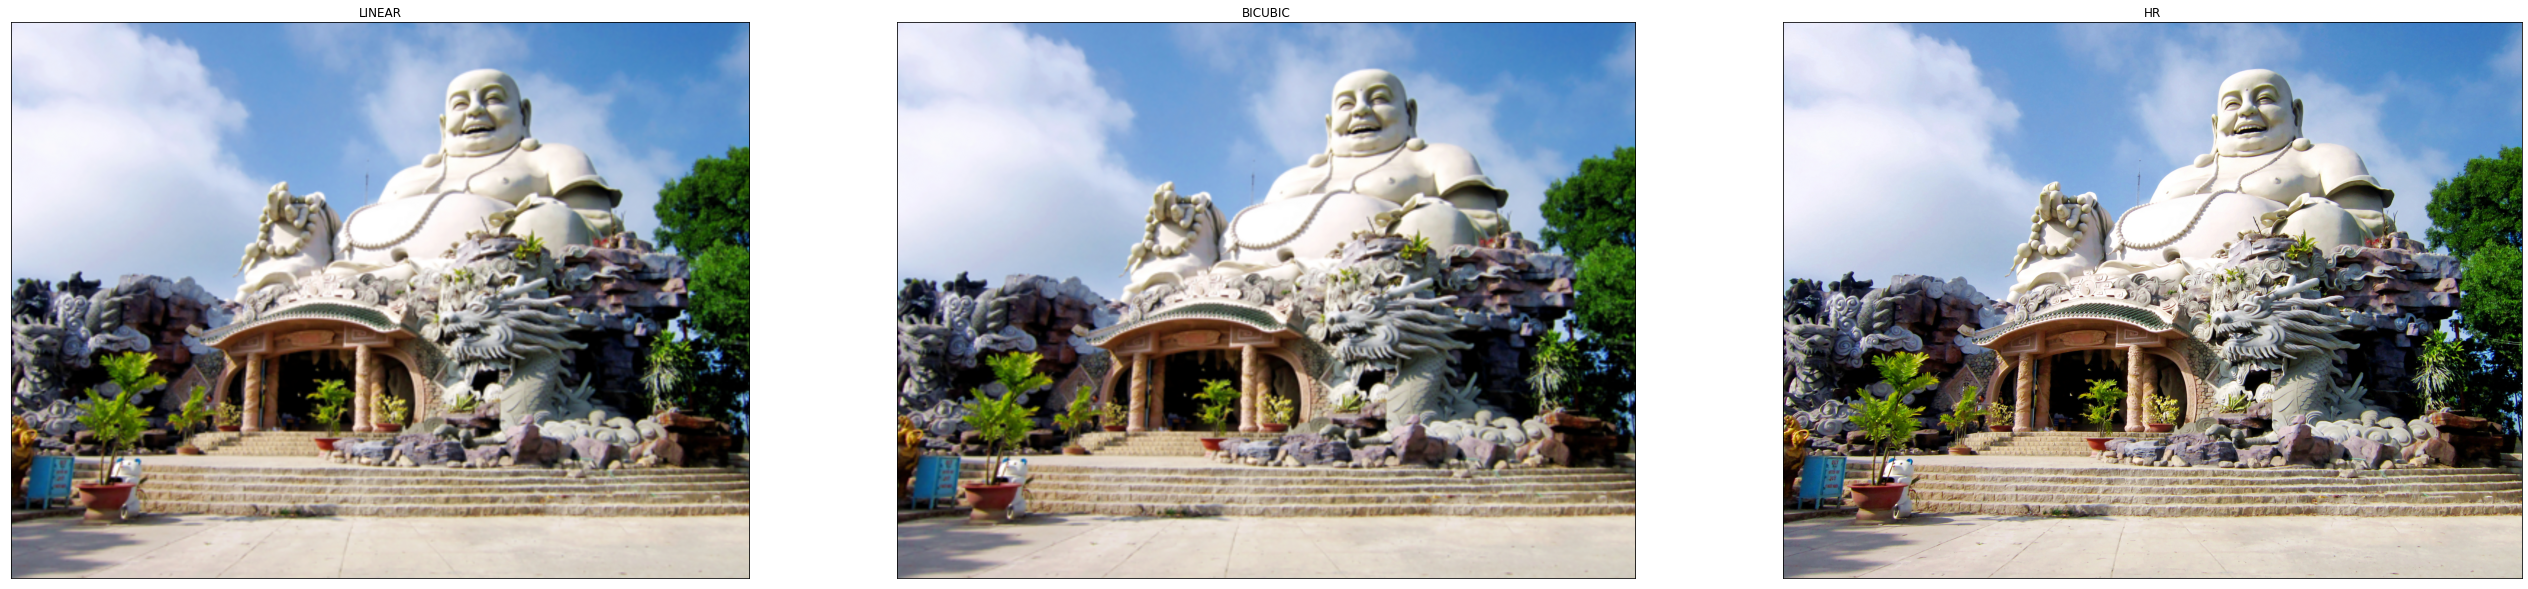
\includegraphics[width=\textwidth,height=\textheight,keepaspectratio]{logos/comparisonstandardresize.png}
     \caption{Comparison of the standard interpolation methods in comparison to the high-resolution image, which is taken from the DIVK dataset \parencite{Agustsson2017}}
    \label{fig:comparison}
\end{figure*}

\par
At first, a \gls{gan} consists of two neural networks: the generator \(G\) and the discriminator
\(D\). The goal of the discriminator is to differ between the training images and the images generated from \(G\). The images are classified as 1 or 0 by the discriminator. Classified as 1 means that the image seems to be real. This leads to a minimisation problem for \(D\) whereas \(G\) is a maximum likelihood function and therefore tries to maximise the objective function, which results in the following formula:

 \[ \min_{G} \max_{D} V(D,G)=\mathbb{E}_{x \sim p_{data}(x)}[log D(x)]+\mathbb{E}_{z \sim p_{z}(z)}[log(1- D(G(z)))] \]
 
The problem with the traditional function is that there is no automatic balance between the generator and the discriminator, and the balance has to be ensured by carefully performing the training. This problem is because the discriminator has a more straightforward job and is thus faster at learning, which results in an underperformance of the generator. This scenario leads to an unpredictable behaviour, and training the same model does not result in the same outcome, as seen in \autoref{fig:failedgan}, where the \gls{gan} reconstructs a given image in the wrong colour in one training. The problem was stated by \cite{salimans2016} that the models hardly achieve the Nash equilibrium, which states when two or more non-cooperative players in a game know each other’s strategy, the best option for each player is to change their strategy. Each model updates its cost individually, which leads to a possible divergence.

\begin{wrapfigure}{l}{0.5\textwidth}
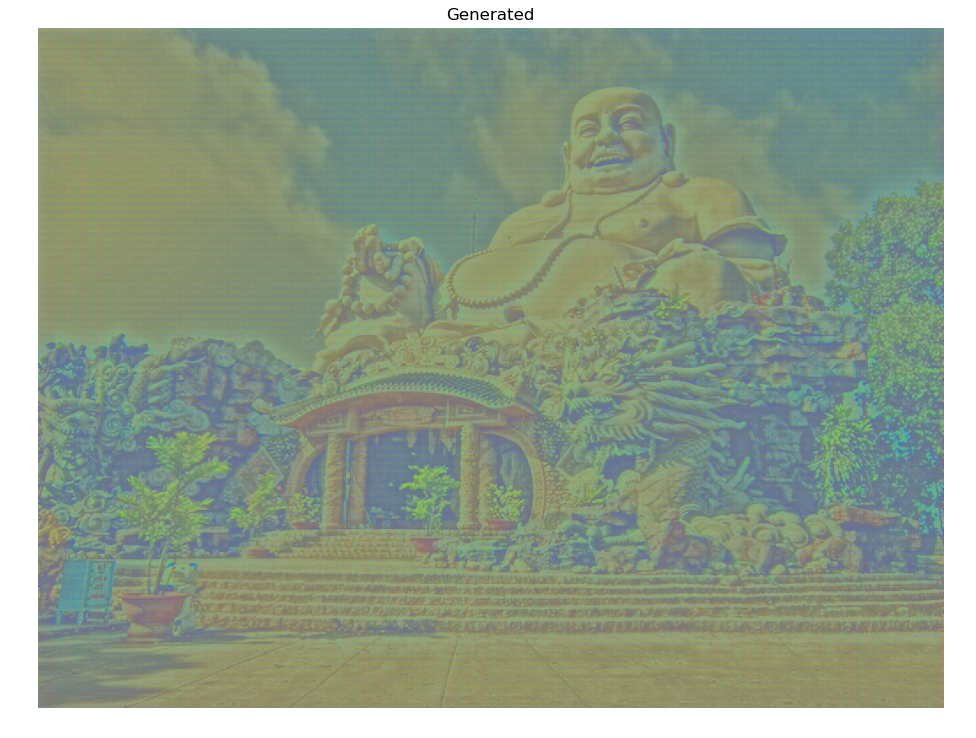
\includegraphics[width=0.9\linewidth]{logos/image_at_epoch_20000.png} 
\caption{Failed training of a \gls{gan}. Image is taken from the DIVK dataset \parencite{Agustsson2017}}
\label{fig:failedgan}
\end{wrapfigure}

\par
Researchers proposed many solutions to keep both in equilibrium. One paper by \cite{ham2020} proposes to pre-train the generator with a \gls{vae}. Since taking the trained weights from one model to a different model is not possible, the decoder of the \gls{vae} and the generator of the \gls{gan} are the same models. This pre-training results in preventing the \gls{gan} to collapse and increases the quality at early epochs. Another possibility is the WGAN named after the Wasserstein metric or Earth-Mover distance (EM distance) distance, which measures the distance between two probabilities \parencite{Vaserstein1969}. In this case, it measures the distance between the generated data distribution \(P_{g}\)and the real data distribution \(P_{r}\) and is defined as

\[W(\mathbb{P}_{r},\mathbb{P}_{g}) = \inf_{\gamma \in \pi(\mathbb{P}_{r},\mathbb{P}_{g})} \mathbb{E}_{(x,y)\sim\gamma}[||x-y||] \]

The WGAN uses this metric as a new loss function of the generator for having a smoother gradient to ensure that the generator learns. The Wasserstein metric works better than the \gls{js} or the \gls{kl}, which are used in a standard \gls{gan}. The \gls{js} is not differentiable at \(\theta\) and the \gls{kl} results in infinity if the two distributions are disjointed. Both algorithms measure the distance of probability distributions as well as the Wasserstein metric. In contrast, the Wasserstein metric gives a reasonable distance. Additionally, the WGAN clamps the weights to a fixed range on every gradient update and uses the RMSProp optimiser instead of the Adam optimiser. Facebook uses a Spectral Normalisation as an extension for the WGAN, which ensures 1-Lipschitz continuity. The spectral normalisation is a weight normalisation technique to stabilise the training of the discriminator \parencite{Miyato2018}. In addition to the adversarial loss, DeepFovea uses more losses like the \gls{lpips} as an extension to the perceptual loss
for detecting distortions and the optical flow loss for stimulating temporal consistency across frames, which results in the follow summary of losses \parencite{Kaplanyan2019}:

\[ L_G = w_{adv}*L_{adv}+w_{LPIPS}*L_{LPIPS}+w_{flow}*L_{flow} \]
\par
The \gls{srgan} project takes a slightly another approach by replacing the MSE content loss of a standard \gls{gan} by a feature extracting method from a pre-trained VGG network, where the name comes from the Visual Geometry Group (Visual Geometry Group 2020) who aim to use a perceptual loss containing two components: a content loss \(l^{SR}_{X}\)and an adversarial loss \(l^{SR}_{GEN}\). The former is usually a pixel-wise MSE loss but often lacks at high-frequency content which results in overly smooth textures \parencite{Ledig2017}. This paper proposes to replace the MSE loss by a VGG loss, which is based on the \gls{relu} activation layers of the pre-trained 19-layer VGG network \parencite{simonyan2015}. This network is a deep convolutional neural network containing 19 layers. It is pre-trained on more than one million images taken from the ImageNet database \parencite{Russakovsky2015} and classifies images into 1,000 object categories such as ‘mouse’, ‘lion’, ‘computer’, ‘TV’ and more. This network originated in the classifying area has thus learned a rich feature representation for a wide range of many images. The adversarial loss is the binary-cross entropy of the generated images classified as real images and the overall sum of generated images in the batch. This results in the following subsequent loss \parencite{Ledig2017}:
\[l^{SR} = l^{SR}_{X} + 0.01 * l^{SR}_{GEN}\]
\par
The overall structural layout of the \gls{srgan} and DeepFovea are different. The \gls{srgan} uses a \gls{resnet} structure as a basic layout. A \gls{resnet} normally consists of several homogeneous blocks containing a skip connection. The skip connection connects the input layer with the output layer in addition to the layers in between. This approach avoids the problem of vanishing gradients which occurs in some cases when the gradient is small enough that the corresponding weight does not change its value, and therefore, the networks stop continuing to learn. By adding the skip connection, the block reuses the activation from a previous layer. During training, this reused value is muted by the actual trained value. The \gls{srgan} uses 16 residual blocks containing two parts. In the first one, a convolutional kernel (Conv2D) layer is followed by batch normalisation and the activation function \gls{prelu}. The second part contains a second Conv2D followed by batch normalisation and the skip connection from the input. Another skip connection surrounds all residual blocks. The approach of the hull of the residual blocks follows a traditional \gls{gan} setup \parencite{Ledig2017}.
\par
In contrast, DeepFovea uses a U-Net setting, which contains a contracting and expansive path, which in this case is an encoder and decoder. This network is based on a fully convolutional network with the main idea to learn the feature mapping of an image and to make it more nuanced than a classic convolutional neural network. For this, the U-Net learns the feature mapping when converting an image into a vector and reuses the mapping to convert the vector back into an image. In this case the degration function is known, as the degration is perfomed in the contracting phase. Therefore, two phases exist that look like a U-shape. In the first phase, which prepares the data to pass through a bottleneck, the spatial information gets reduced, and the feature information increases, which is called the contracting phase. In the expansive phase, both pieces of information are combined, as each block gets the input of the former expansive block and the corresponding contracting block. This setup ensures that the correct feature mapping which has been learned is used for the reconstruction. This process requires that the amount of expansive block is the same as the contraction blocks \parencite{ronneberger2015}. Furthermore, DeepFovea uses four residual blocks for the contracting, one connecting residual block as the bottleneck and four temporal blocks in the expansive phase. Each residual block contains two 3D convolutional blocks followed by an \gls{elu} activation function. Similarly to the \gls{srgan}, the residual block uses a skip connection from the input to the average pooling. The temporal blocks contain again two 3D convolutions, where the first one is followed by layer normalisation, an \gls{elu} activation and recurrent connection to the input. The second Conv3D has an \gls{elu} activation again and is followed by a bilinear upsample. The temporal block also contains a skip connection from the input to the upsample layer. The input of this network is a 5D sparsified matrix that contains more information in the foveated area and less information the further away from this region. This input requires using the 3D convolutional layers. This fact makes it hard to reconstruct this neural network for this project, because in this setting, only a three-dimensional image exists as an input. Therefore, the \gls{srgan} was used as the ground structure.

\begin{figure*}
    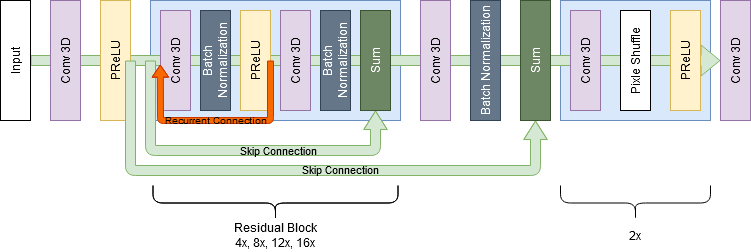
\includegraphics[width=\textwidth,height=\textheight,keepaspectratio]{logos/Generator.png}
     \caption{Generator}
    \label{fig:generator}
\end{figure*}

\par
As the generator from the \gls{srgan} works well in terms of producing quality images, the \gls{srgan} is taken as basis for further development. The first difference is inside a residual block where it becomes necessary to adjust the network from performing superresolution from images to videos. In this case, the idea of DeepFovea to use recurrent connections is implemented. Moreover, the more complicated and extensive a network is, the slower it becomes during live inference. Thus, the different configurations of the residual blocks are compared against each other. The generator is shown in \autoref{fig:generator}, with 4 to 16 possible residual blocks and the recurrent connection as an LSTM layer, which also requires to upgrade the Conv2D to a Conv3D as a dimension namely time is added. Alternatively, the training process and the loss function are different. First, the generator is pre-trained with an autoencoder as proposed by \cite{ham2020}. Second, the loss function is that of the DeepFovea’s as explained to comprehend the missing residual blocks. In particular, the neural network uses the combination of \gls{lpips} loss and optical flow loss in addition to the adversarial loss as proposed in the WGAN. The weights are the same as proposed by Facebook, namely: \(w_{adv}=1, w_{LPIPS}=100\). The optical flow had to be skipped due to hardware constraints. Additionally, the weights are clamped after each training process and the gradients are optimised by the RMSProp optimiser.
\par 
The discriminator has no impact on the latency, because it is not involved in the live inference and can be as large as needed. Therefore, the generators’ counterparty is the original from the \gls{srgan} with the improvements of the spectral normalisation. The resulting discriminator is presented in \autoref{fig:discriminator} \parencite{Ledig2017}.

\begin{figure*}[htbp]
    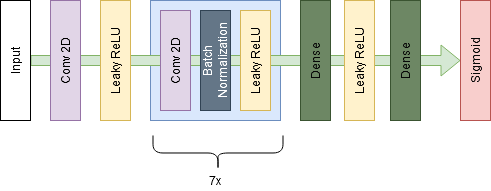
\includegraphics[width=\textwidth,height=\textheight,keepaspectratio]{logos/Discriminator.png}
     \caption{Discriminator}
    \label{fig:discriminator}
\end{figure*}

\par
In conclusion, building and training a \gls{gan} is challenging. Therefore the \gls{srgan} is taken as a basis and for further development and is improved by training techniques as presented in this chapter. This method guarantees a minimum of quality as two functional neural networks are combined. In the next chapter, it is determined how the \gls{gan} performs in terms of quality and latency in comparison to standard resizing techniques. Moreover, the general concept of the implementation, presented in this chapter, is tested.